\documentclass[11pt,a4paper]{jsarticle}
%
\usepackage{amsmath,amssymb}
\usepackage{bm}
\usepackage[dvipdfmx]{graphicx}
\usepackage[dvipdfmx]{color}
\usepackage{ascmac}
\usepackage{listings}
%
\setlength{\textwidth}{\fullwidth}
\setlength{\textheight}{40\baselineskip}
\addtolength{\textheight}{\topskip}
\setlength{\voffset}{-0.2in}
\setlength{\topmargin}{0pt}
\setlength{\headheight}{0pt}
\setlength{\headsep}{0pt}
%
\newcommand{\divergence}{\mathrm{div}\,}  %ダイバージェンス
\newcommand{\grad}{\mathrm{grad}\,}  %グラディエント
\newcommand{\rot}{\mathrm{rot}\,}  %ローテーション
%
\title{レポート課題11}
\author{05-191009 奥村真司}
\date{}
\begin{document}
\maketitle
%
%
\section*{問1}
\subsection*{考察}
以下のように探索が無限ループするため期待どおりに動かない。
$$ancestor(kobo,iwao)\ \ \ \rightarrow$$
$$ancestor(Z_1,iwao),parent(kobo,Z_1)\ \ \ \rightarrow$$
$$ancestor(Z_2,iwao),parent(Z_1,Z_2),parent(kobo,Z_1)\ \ \ \rightarrow...$$
前回の授業でやったとおり、
\begin{lstlisting}[basicstyle=\ttfamily\footnotesize, frame=single]
ancestor(X,Y) :- parent(X,Z),ancestor(Z,Y).
ancestor(X,Y) :- parent(X,Y).
\end{lstlisting}
とすればZが決まりやすく、期待通り動作する。
\section*{問2}
\subsection*{考察}
探索は以下の画像のように進む。\\
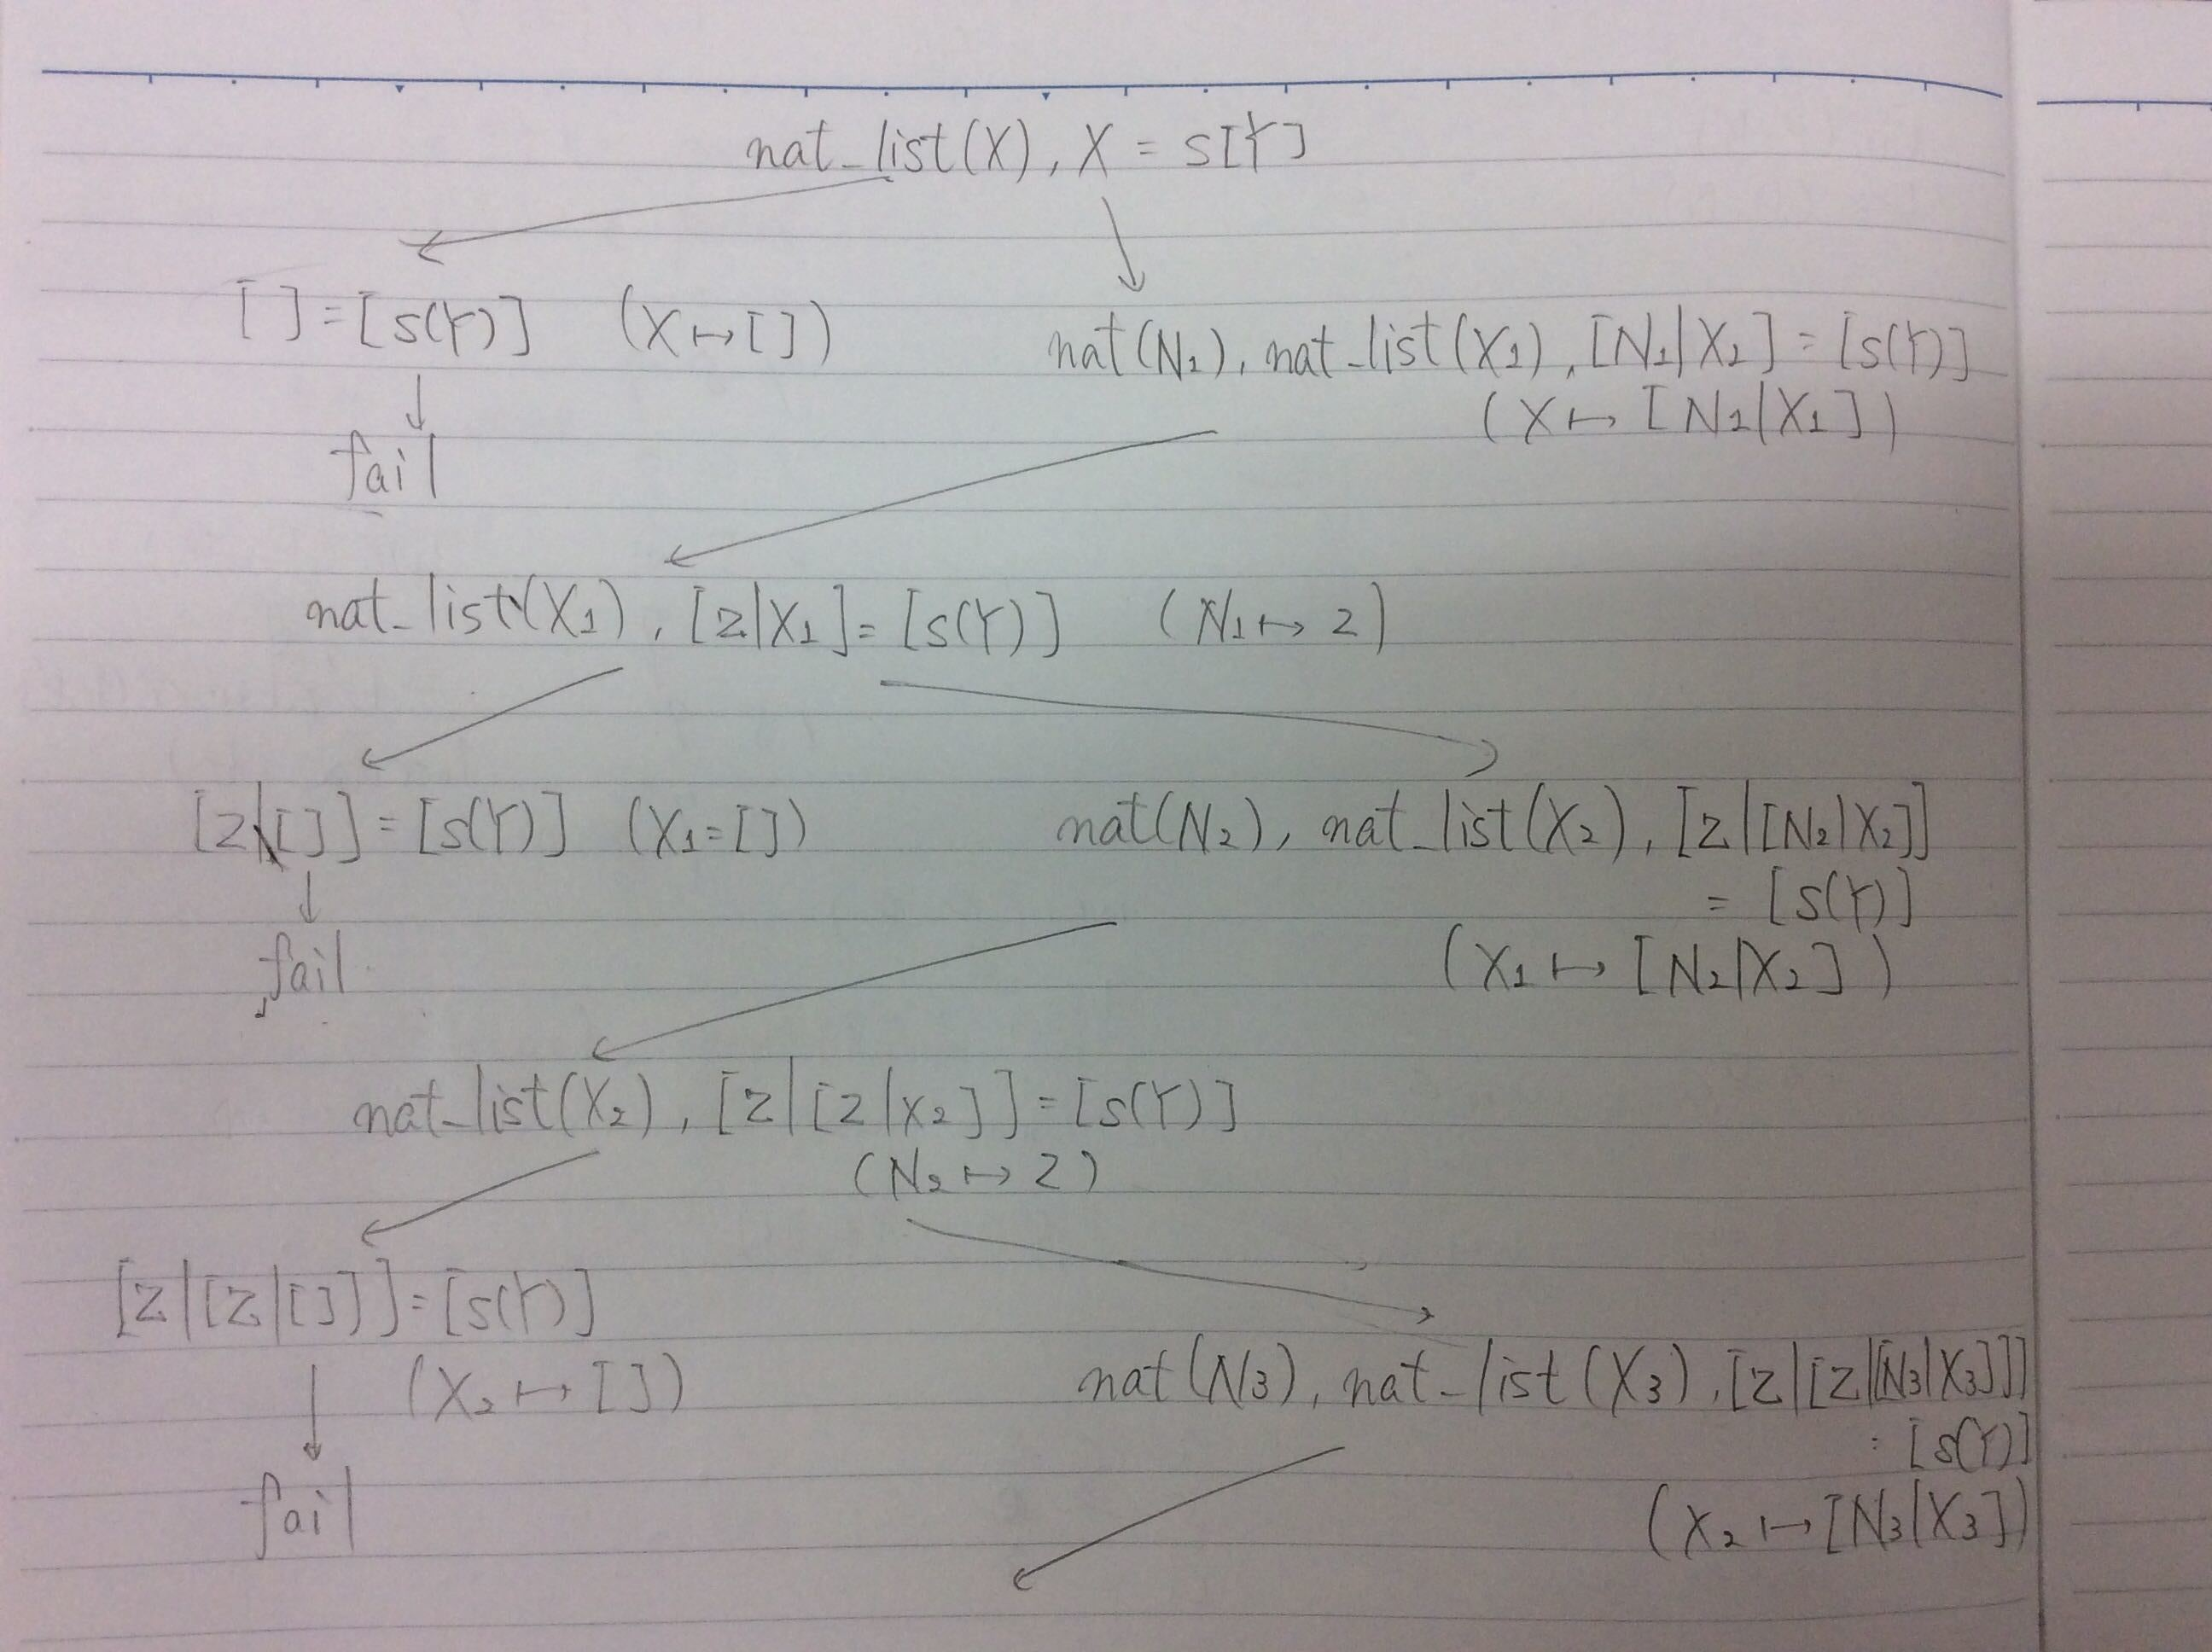
\includegraphics[width=14.5cm]{problem2.jpg}\par
図のように、$nat(N_k),nat\_list(X_k),[z|[z|..|[N_k|X_k]..]]]]=[s(Y)]$
の形の状態が現れ続け、無限に探索が終わらない。
以下のように
\begin{lstlisting}[basicstyle=\ttfamily\footnotesize, frame=single]
nat(z).
nat(s(N)) :- nat(N).
nat_list([]).
nat_list([N|X]) :- nat_list(X),nat(N).
\end{lstlisting}
として(4行目のnat,nat\_listの順序を入れ替えた)リストの要素が自然数かチェックするより先にリストの形を決めてやることで探索範囲をせばめてやると、期待通り動作するようになった。
\section*{問3}
\subsection*{動作例}
\begin{lstlisting}[basicstyle=\ttfamily\footnotesize, frame=single]
?- ['family.pl'].
true.

?- win(a,[e,e,e,e,e,e,e,e,e]).
false.

?- lose(a,[e,e,e,e,e,e,e,e,e]).
false.

?- win(a,[a,e,e,b,e,e,e,e,e]).
true .

?- win(a,[e,e,e,b,a,e,e,e,e]).
true .

?- win(a,[e,a,e,b,e,e,e,e,e]).
true .
\end{lstlisting}
\subsection*{考察}
実装にあたって定義したPredicateの説明をする。
$$end(P,B) \Leftrightarrow 盤面BでプレイヤーPがすでに勝っている(3つならべている)$$ 
$$enemy(P,Q) \Leftrightarrow Pの相手がQ$$
$$next(P,B,C) \Leftrightarrow Pの手番で盤面Bの状態から盤面Cの状態になりうる$$
$$notfull(B) \Leftrightarrow 盤面Bで空きマスがある$$
を実装した。
loseの実装の際に全称量化子が必要になるが、Prologで自然に書けるPredicateは限定量化子のついた形だと思ったので先頭に2重否定をつけ、内側の否定を全称量化子の中に入れて量化子を存在量化子に変えて実装した。すなわち、loseで
$$next(P,B,C)なる任意の局面Cについてwin(Q,C)$$
を
$$(next(P,B,C)なるある局面Cが存在してwin(Q,C)でない)でない$$
とした。これらを用いてwin,loseは
\begin{lstlisting}[basicstyle=\ttfamily\footnotesize, frame=single]
win(P,B) :- end(P,B).
win(P,B) :- enemy(P,Q),\+end(Q,B),next(P,B,C),lose(Q,C).
notwin(P,B) :- \+ win(P,B).
notlose(P,Q,B) :- next(P,B,C),notwin(Q,C).
lose(P,B) :- enemy(P,Q),end(Q,B).
lose(P,B) :- enemy(P,Q),\+end(P,B),notfull(B),\+ notlose(P,Q,B).
\end{lstlisting}
のように実装できた。
このPredicateでは探索していくので順次未決定な部分が決まっていく。なので否定はあまり深く考えずに述語論理と対応させて用いた。
動作例のはじめの2つから、先手後手ともに必勝法がないことがわかる。
また授業スライド内の各盤面状態が先手必勝であることも確認できた。
\section*{発展1}
\subsection*{動作例}
\begin{lstlisting}[basicstyle=\ttfamily\footnotesize, frame=single]
?- rule nat(z).
?- rule nat(s(X)) :- nat(X).
?- query nat(X).
X = z
;
X = s(z)
;
X = s(s(z))
;
X = s(s(s(z)))
;
X = s(s(s(s(z))))
;
X = s(s(s(s(s(z)))))
;
X = s(s(s(s(s(s(z))))))
;
X = s(s(s(s(s(s(s(z)))))))
.
?- rule male(koji).
?- rule parent(kobo,koji).
?- rule father(X,Y) :- parent(X,Y),male(Y).
?- query father(kobo,Z).
Z = koji
;
false.
?- rule add(z,Y,Y).
?- rule add(s(X),Y,s(Z)) :- add(X,Y,Z).
?- query add(s(z),X,X).
false.
?- rule append([],Y,Y).
?- rule append([A|X],Y,[A|Z]) :- append(X,Y,Z).
?- rule concat([X|[]],X).
?- rule concat([X|Y],Z) :- concat(Y,W),append(X,W,Z).
?- query append([1,2,3],[4,5],Z).
Z = [1, 2, 3, 4, 5]
;
false.
?- query append(X,Y,[1,2,3,4,5]).
Y = [1, 2, 3, 4, 5]
X = []
;
Y = [2, 3, 4, 5]
X = [1]
;
Y = [3, 4, 5]
X = [1, 2]
;
Y = [4, 5]
X = [1, 2, 3]
;
Y = [5]
X = [1, 2, 3, 4]
;
Y = []
X = [1, 2, 3, 4, 5]
;
false.
?- query concat([[1],[2,3,4]] ,X).
X = [1, 2, 3, 4]
;
false.
?- rule in(X,[X|Y]).
?- rule in(X,[Y|Z]) :- in(X,Z).
?- rule choose([X|Y],Y,X).
?- rule choose([A|X],[A|Y],Z) :- choose(X,Y,Z).
?- rule hamilton(V,E) :- choose(V,Rem,Start),hamiltonsub(Rem,E,Start).
?- rule hamiltonsub([],X,Y).
?- rule hamiltonsub(V,E,Now) :- choose(V,Rem,Next),in([Now|[Next|[]]],E),
hamiltonsub(Rem,E,Next).
?- query hamilton([1,2,3,4],[[1,2],[2,3],[3,4],[4,1]]).
true.
;
true.
;
true.
;
true.
;
false.
?- query abcd.
Undefined procedure.
?- query a([,
Parse Error.
?- $
Failure Unknown Token: $
\end{lstlisting}
\subsection*{考察}
Prologライクな論理型言語のインタプリタをレクサー、パーサーも含め実装した。動作例のように、前回の授業で扱ったものや課題の解答で自分で作成したものについて、期待通りに動作することがわかった。addの例では出現検査をちゃんと行えていることが確認できた。この動作例における入力データはverify.pl内にある。
\subsubsection*{定数、項、述語などの扱い}
実装を始めるにあたってまず定数、項、述語などのデータをどう扱うかを考えた。これらの文法はPrologと同じようにした。syntax.ml内でこれらの型は下のように定義されている。
\begin{lstlisting}[basicstyle=\ttfamily\footnotesize, frame=single]
type name = string 
type var = int

type term =
  | EConst of name
  | EFnSymb  of name * (term list)
  | EVar of name
  | ECons of term * term
  | ENil

type fact = EPdSymb of name * (term list)

type rule = fact * (fact list)

type command =
  | CRule    of rule
  | CQuery   of fact list
  | CCont
  | CExit

type subst = (name * term) list

type constraints = (term * term) list
\end{lstlisting}
termが授業スライドでの項にあたるもので、定数がEConst,ファンクタがEFnSymb(Function Symbol),..というようになっている。述語(項,項,...)をfactという名前にした(この形式にfactという名前をつけただけでこれが意味的にfactとは限らない。例えば問い合わせでのゴールのリストはfact listである。)。述語(項,項,...) :- 述語(項,項,...),述語(項,項,...),...がruleである。\par
ルールの読み込みと問い合わせの区別は入力の先頭にruleかqueryとつけることを要求することで実現した。queryではそこまでに入力されたrule全てを用いてSLD導出を探索する。
\subsubsection*{探索}
次に探索について説明する。授業スライドにもあるとおりSLD導出を探索しているが、swi-prologと異なり幅優先探索(BFS)で探索し、単一化時に出現検査を行うようにした。\par
ゴールのリストの先頭とルールを単一化する際に、入力された通りの変数名を用いると変数名がかぶっているときに正しく単一化できないので、ルールを用いるたびに内部の変数名をすべてuniqueなものに置き換えている。がsyntax.ml内のconvert\_$****$という関数群はこの置き換えを行うための補助関数である。
例えば$\texttt{father(X,Y) :- parent(X,Y),male(Y)}$というruleなら、$\texttt{father(\_1,\_2) :- parent(\_1,\_2),male(\_2)}$のように置き換えられる。同じルールでも置き換えを行うたびに別のものになる。\par
探索の各状態はfact list型のゴールのリストとsubst型の置き換えの組になっている。
BFSの実現方法について説明する。BFSはQueueを用いて行った。計算量的には好ましくないが、listをqueueとみなし@で後ろにつなげることでpushを、先頭の取り出しはパターンマッチで行っている。eval内のnextという関数は探索状態と仕様するルールを受け取って、ゴールリストの先頭とルールが単一化可能なら次の状態のsigletonリストを,不可能なら空リストを返す関数であり、$\texttt{List.concat (List.map (fun r -> next q r) rules)}$とすることで現在の状態qからルールrulesを用いて遷移可能な状態のリストが得られる。これをqueueの後ろに@でつないでいる。これを@で前につなぐように変更するだけで簡単にDFSにすることもできる。解が見つかったらその時点でのqueueの状態も一緒に返してやることで、続きからの探索も可能になっている。
\subsubsection*{その他こだわりポイント}
以下は課題の出題意図とは直接的には関係ないと思われるがこだわった点について説明する。
\begin{itemize}
	\item リストの[x,y,z]の入出力形式のサポート\par
	はじめはコンスの形のみサポートしていたが非常に入力しづらいので[x,y,z]の形式をサポートした。これが意外と思考を要したのでそれについて説明する。$\texttt{[a|b]}$を以下の画像のように捉えることで、termの構造はEConsによる完全二分木と捉えることができる。[x,y,z],[x,y,z$|$w]は下のような木構造を表すことから、[x,y,z]は[x,y,z$|$[]]の省略形と思える。
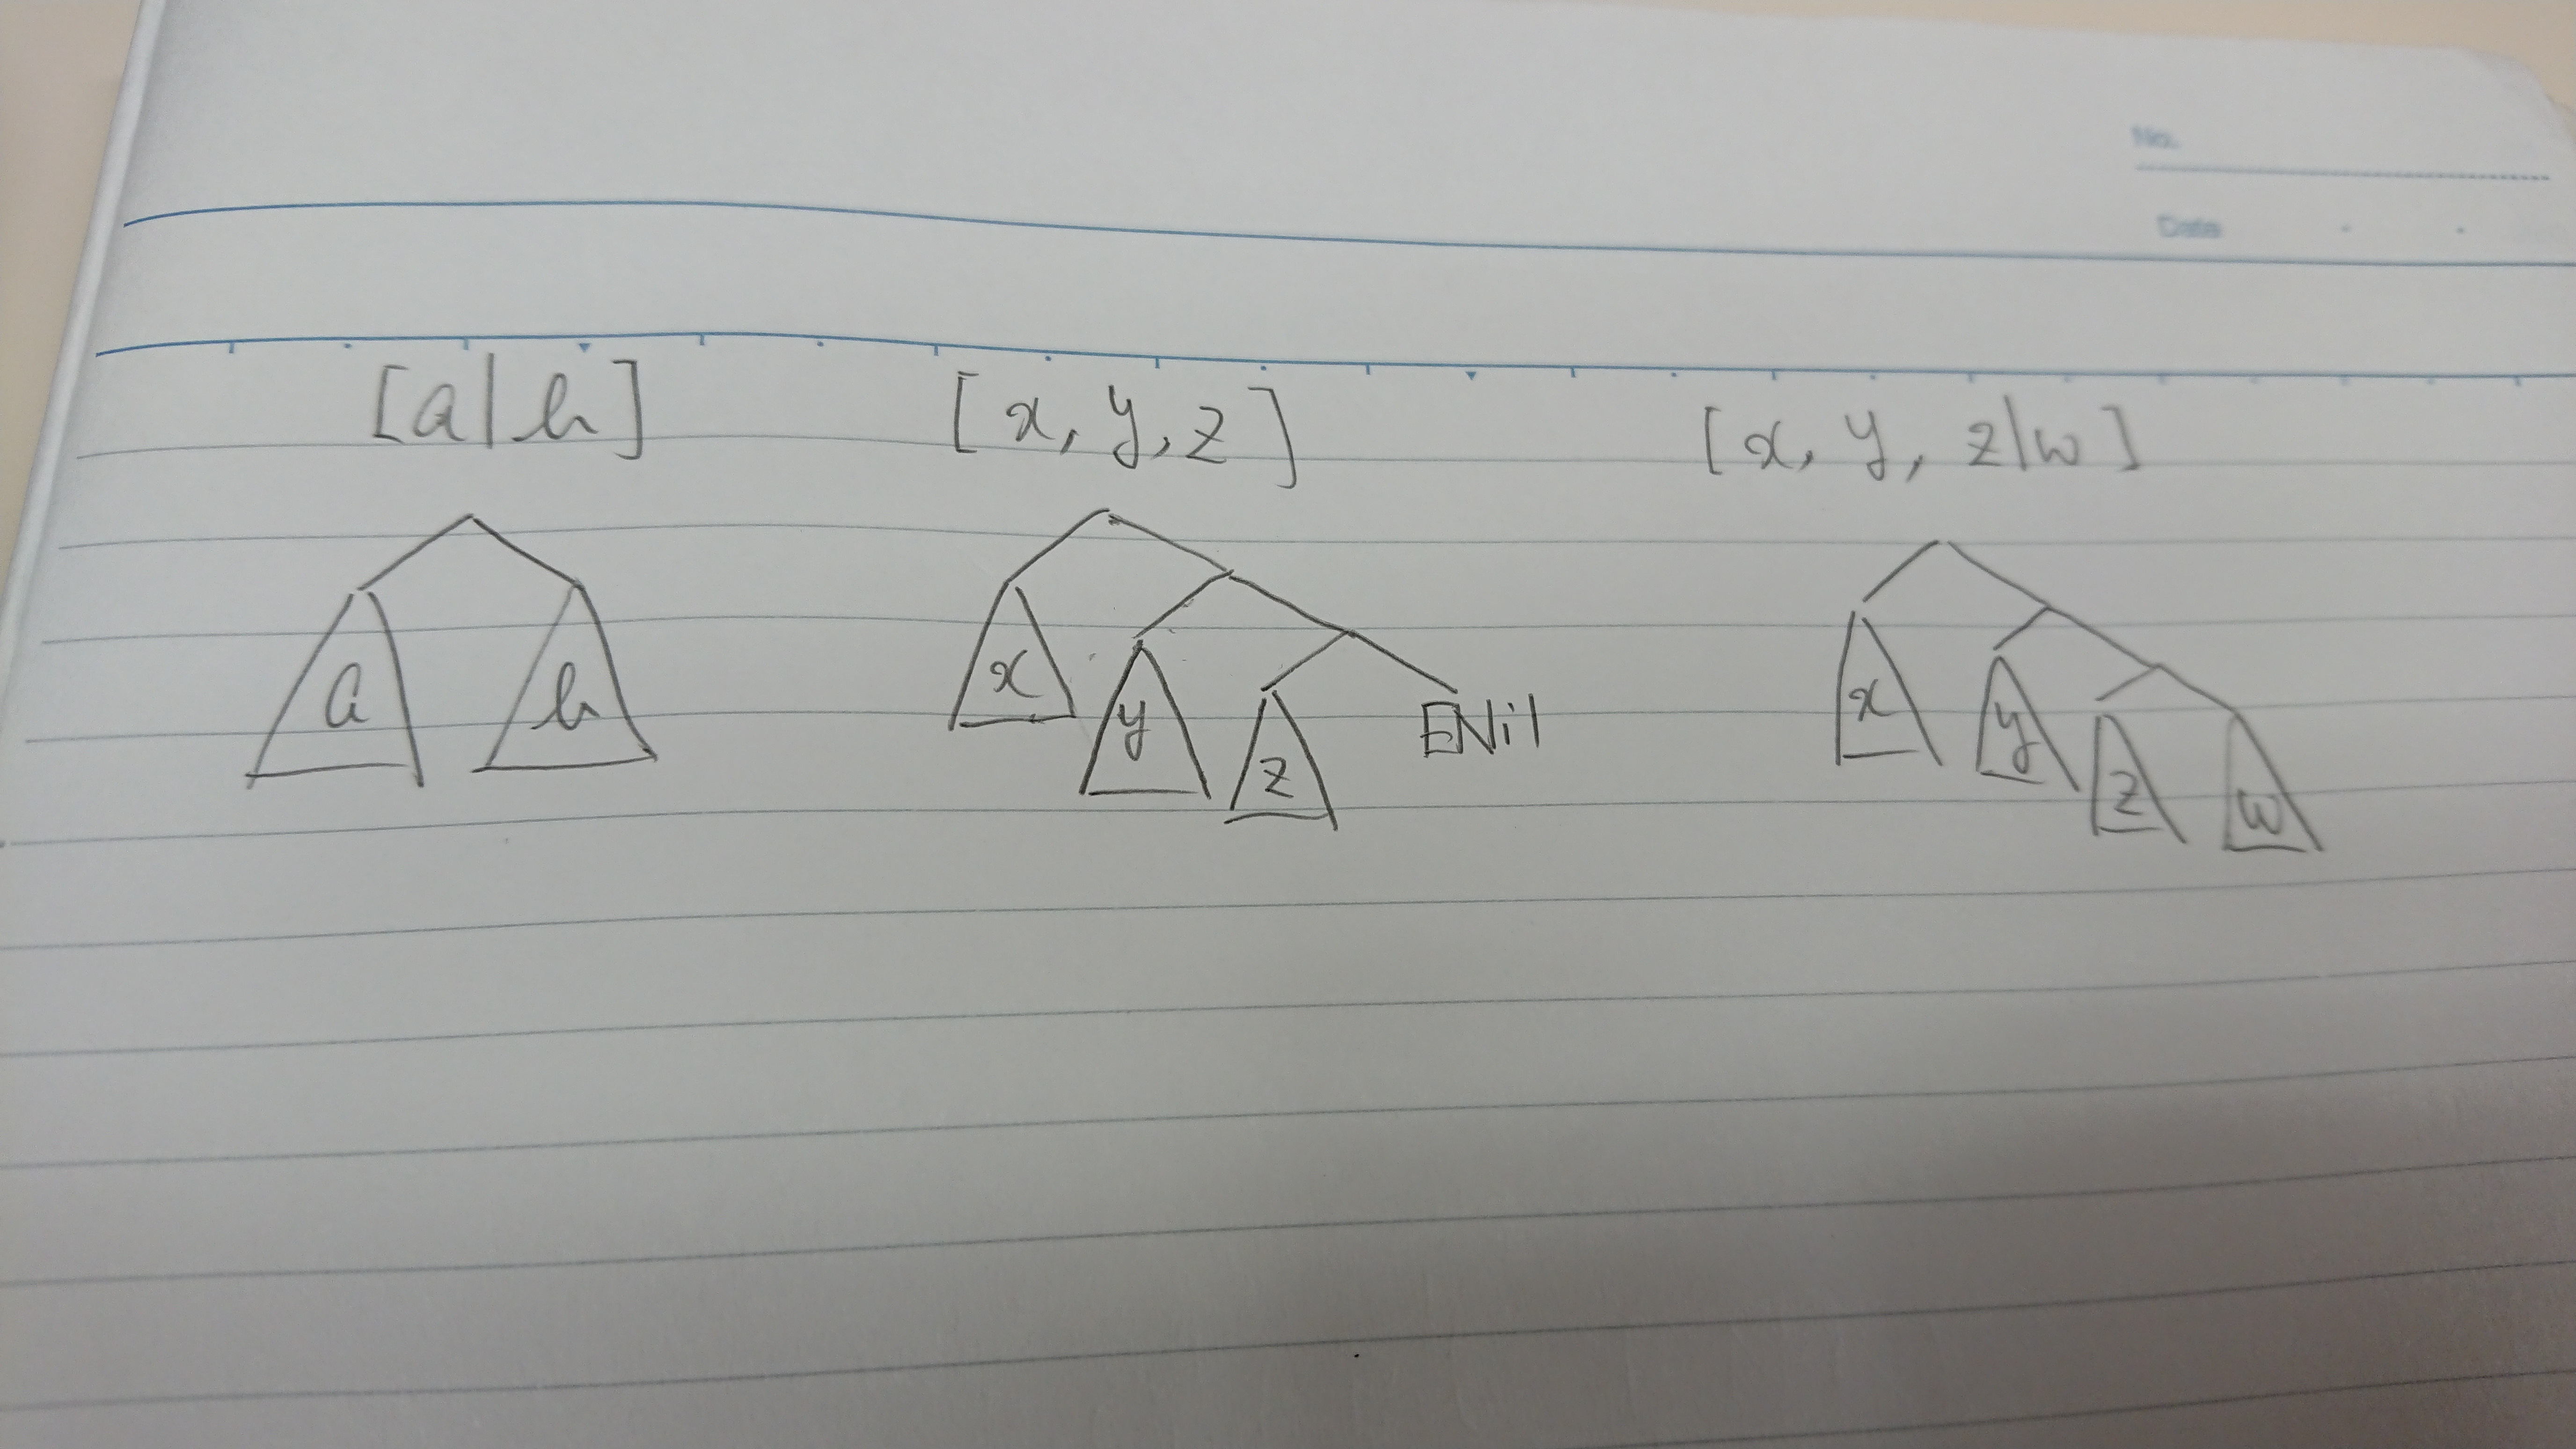
\includegraphics[width=14.5cm]{LsitTree.jpg}\par
	よって、最後の要素で場合分けして考えることでParserは以下のように書けた。
\begin{lstlisting}[basicstyle=\ttfamily\footnotesize, frame=single]
atomic:
  | SYMBID { EConst($1) }
  | NUMBER { EConst($1) }
  | VARID  { EVar($1) }
  | list   { $1 }
;

atomics:
  | list_last { $1 }
  | atomic COMMA atomics { ECons($1,$3) } 
;

list_last:
  | atomic { ECons($1,ENil) }
  | atomic BAR atomic { ECons($1,$3) }
;

list:
  | NIL { ENil }
  | LBRACKET atomics RBRACKET { $2 }
;
\end{lstlisting}
出力も、カンマを出力すべきかどうかをパターンマッチで場合わけして以下のように書くことができた。
\begin{lstlisting}[basicstyle=\ttfamily\footnotesize, frame=single]
let rec print_term t = 
  match t with
  | EFnSymb (id,tl) -> print_name id;
                       if tl=[] then ()
                                else (print_string "(";
                                      print_term_list tl;
                                      print_string ")")
  | EVar id -> print_name id
  | ECons (x,y) -> print_list t
  | ENil -> print_string "[]"
  | EConst x -> print_name x 
and print_term_list tl = 
  match tl with
  | [] -> ()
  | t::rest -> print_term t;
               (if (rest <> []) then (print_string ",") 
                                else ());
               print_term_list rest
and print_list t =
  print_string "[";
  print_list_inner t;
  print_string "]"
and print_list_inner t =
  match t with
  | ECons (x,(ECons(y,z))) -> print_term x;
  		   	  print_string ", ";
  		   	  print_list_inner (ECons (y,z))
  | ECons (x,ENil) -> print_term x
  | ECons (x,y) -> print_term x;
  		   print_string " | ";
  		   print_term y
  | _ -> () (* Error *)
\end{lstlisting}
	\item エラー\par
	動作例の最後から3つめのように、全く定義されていない述語についての問い合わせが来た場合に、閉世界仮説的にはfalse.でいいのではないかと思ったが、swi-prologではUndefined procedureというエラーが出るようになっていたのでそれを採用し、チェックするようにした。
	動作例の最後のあたりのように、レクサーやパーサーのエラーも含めエラーが発生しても処理系はエラーメッセージを出力して次の入力を待ち、終了しないようにした。なおエラー出力およびfalse.はbashで赤文字で出力されるようにした。
\end{itemize}
\end{document}
